\section{Le schéma}
\begin{figure}[H]
    \centering
    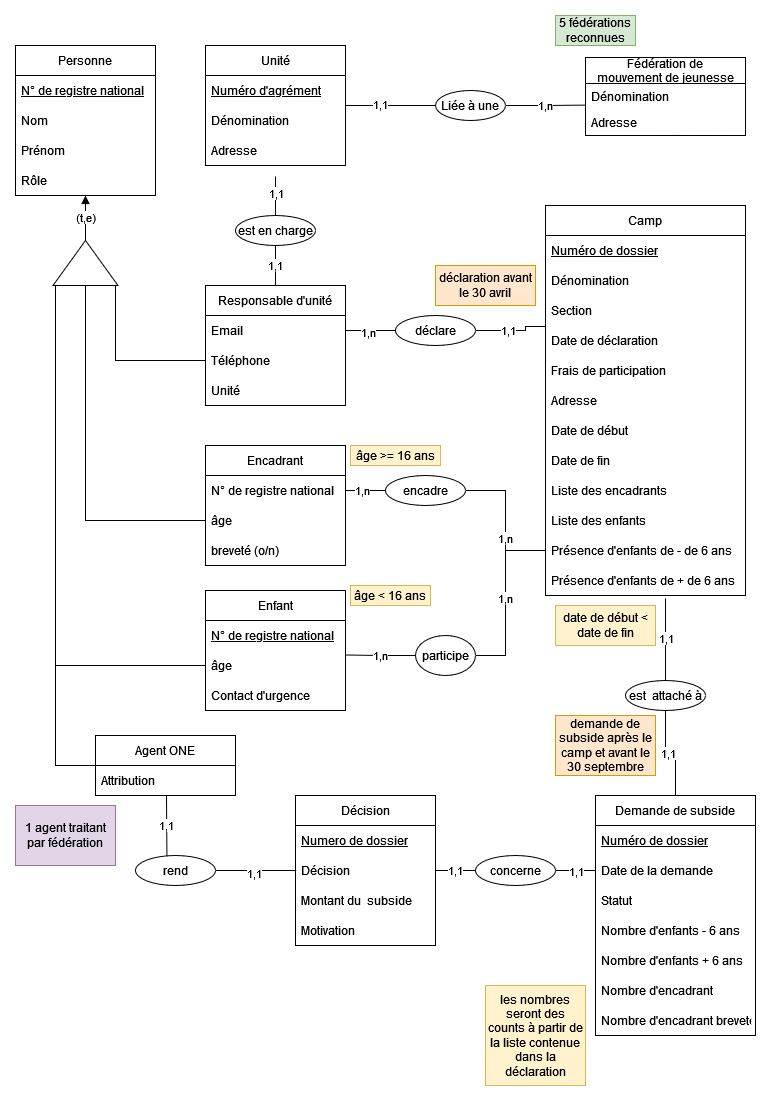
\includegraphics[height=17cm]{Pictures/modele_ea.jpg}
    \caption{Modèle entités-associations}
    \label{fig:modele_ea}
\end{figure}

\subsection{Les entités: quelques explications}

\subsubsection{Fédération de mouvement de jeunesse}
Il n'existe que cinq fédérations de mouvement de jeunesse (cf. point \ref{fmj}). 

\subsubsection{Unités}
Chaque unité appartient à une seule fédération de mouvement de jeunesse. Il y a également plusieurs sections au sein d'une unité, mais la modélisation n'est pas pertinente pour notre domaine d'application. Une unité organise plusieurs camps; une par section environs. L'information de section figure dans l'entité camp. 


\subsubsection{Correspondant: chef d'unité}
Il s'agit de la personne de contact de l'unité. L'adresse de correspondance est parfois différente de celui du Pouvoir organisateur (qui est l'adresse officielle). Une adresse mail et un numéro de téléphone est également demandé. 

\subsubsection{Déclaration de camp}
Le chef d'unité déclare le:
\begin{itemize}
    \item \textbf{nom du camp}: il s'agit parfois du thème du camp ou du lieu-dit (une prairie, un endroit proche d'une rivière, etc.)
    \item \textbf{l'adresse} de ce camp
    \item quelques \textbf{caractéristiques d'accueil}, comme par exemple la tranche d'âge accueillie, les frais de participations demandées aux parents, etc.
    \item les \textbf{dates du camp}
    \item et enfin une \textbf{liste des encadrants chef} et une liste \textbf{des animés enfants}.
\end{itemize}

La déclaration doit parvenir à l'ONE avant le 30 avril. L'ONE envoie ensuite un formulaire de demande de subsides avec le numéro du dossier du camp.

Le chef déclare les camps au nom de l'unité qui les organise. Les déclarations sont donc liées à l'unité dans notre base de données. Une unité organise un ou plusieurs camps généralement en fonction du nombre de ses sections. 


% supprimé 
%\subsection{Le responsable qualifié}
%Le responsable qualifié sera la personne de contact et physiquement sur place pour les visites des coordinatrices accueil. Il fait parti du personnel d'encadrement du camp et n'est pas nécessairement le correspondant de l'unité.


\subsubsection{La demande de subsides}
Lorsque les données dans la déclaration sont complètes (liste d'enfants et liste d'encadrant complétées) et que le camp est passé, le responsable d'unité peut faire une demande de subside. 
Les données demandées sont le nombre d'enfants et de chefs l'identité et la caractéristique des enfants (âge, porteur de handicap, en situation défavorisée, etc.) et des chefs ( breveté). 


Un bouton dédié créera la demande de subsides. L'agent ONE traitant pourra alors encoder une décision de subside.

La demande de subsides intervient après le déroulement du camp d'été et doit être envoyé avant le 30 septembre. 



La demande de subsides est donc liée directement à la déclaration et est traité par un agent traitant qui rend une décision. 

\subsubsection{Agent traitant ONE}
Il y a un agent traitant par dossier de fédération. Un même agent s'occupe donc de l'ensemble des dossiers Patros, un autre des dossiers Guides, etc. 


\subsubsection{Décision concernant la demande de subsides}
La demande de subsides débouche sur une décision de la part de l'ONE (agent traitant). En fonction de la décision, une somme de subsides est accordée pour le camp.


\subsection{Héritage is-a}

\subsubsection{Personne}
Dans le schéma conceptuel, les responsables d'unité, les enfants, animateurs et agent ONE sont des personnes. Un super-entité Personne rassemble les informations d'identification personnelle. 
